% A paper in the layout of NIPS 2017's style — made up, after "Attention Is
% All You Need" (arXiv:1706.03762) — with what Reflow once read badly in it:
% a notice set over the title; a byline set as a grid, each name over its
% institution and its address in a column of its own; a footnote on every
% name that says, sentence by sentence, who did what; paragraphs parted by
% space rather than an indent; a sum in a footnote; a table whose cells are
% all O(n) and no figures; a figure whose label the clip leaves out; and an
% "Author Contributions" section that names the authors by their initials.
% Rebuilt with: pdflatex nips-grid-figure.tex && pdflatex nips-grid-byline.tex
% (texlive-latex-recommended).
\documentclass[10pt]{article}
\usepackage[T1]{fontenc}
\usepackage[margin=1.5in]{geometry}
\usepackage{amsmath,amssymb,booktabs,graphicx,xcolor}
\usepackage{hyperref}
\setlength{\parindent}{0pt}
\setlength{\parskip}{5.5pt}
\renewcommand{\thefootnote}{\fnsymbol{footnote}}
\title{{\normalsize\color{red}Provided proper attribution is provided, Northfield Research grants permission to reproduce the tables and figures in this paper for scholarly works.}\\[1em]\rule{\linewidth}{2pt}\\[0.5em]\textbf{Attention Is What Northfield Needs}\\\rule{\linewidth}{0.5pt}}
\author{
\begin{tabular}[t]{c}\textbf{Ada Lindqvist}$^*$\\Northfield Brain\\\texttt{adal@nf.example.com}\end{tabular}\hfill
\begin{tabular}[t]{c}\textbf{Tomas Okafor}$^*$\\Northfield Research\\\texttt{tko@nf.example.com}\end{tabular}\hfill
\begin{tabular}[t]{c}\textbf{Mira Castell}$^{*\dagger}$\\University of Eastmoor\\\texttt{mira@eastmoor.example.edu}\end{tabular}\\[1.5em]
\begin{tabular}[t]{c}\textbf{\L{}ukasz Borowski}$^*$\\Northfield Brain\\\texttt{lukaszb@nf.example.com}\end{tabular}\hfill
\begin{tabular}[t]{c}\textbf{Ravi Anand}$^{*\ddagger}$\\\texttt{ravi.anand@mail.example.org}\end{tabular}
}
\date{}
\begin{document}
\maketitle
\footnotetext[1]{Equal contribution. Listing order is random. Mira proposed replacing recurrence with attention and started the effort to evaluate this idea. Ada, with Ravi, designed and implemented the first models and has been crucially involved in every aspect of this work. Tomas proposed scaled attention and became the other person involved in nearly every detail. Lukasz and Mira spent countless long days designing various parts of the codebase.}
\footnotetext[2]{Work performed while at Northfield Brain.}
\footnotetext[3]{Work performed while at Northfield Research.}
\renewcommand{\thefootnote}{\arabic{footnote}}\setcounter{footnote}{3}
\begin{abstract}
The dominant models are based on recurrent networks that include an encoder and a decoder. We propose a new simple architecture based solely on attention, dispensing with recurrence entirely, and show it is better and faster to train on two translation tasks.
\end{abstract}
\section{Model}
We call our particular attention scaled attention. The input consists of queries and keys of dimension $d_k$, and values of dimension $d_v$. We compute the dot products of the query with all keys, divide each by $\sqrt{d_k}$, and apply a softmax function to obtain the weights on the values.

In practice, we compute the attention function on a set of queries simultaneously, packed together into a matrix. The keys and values are also packed together into matrices, and the outputs are computed at once for all of them. This paragraph runs on for a few more lines of text, so that the body of the page is measured as justified text by the reader, which is what it is.

While for small values of $d_k$ the two mechanisms perform similarly, additive attention outperforms dot product attention without scaling for larger values of $d_k$. We suspect that for large values of $d_k$ the dot products grow large in magnitude, pushing the softmax into regions where it has extremely small gradients\footnote{To illustrate why the dot products get large, assume that the components of $q$ and $k$ are independent random variables with mean 0 and variance 1. Then their dot product, $q \cdot k = \sum_{i=1}^{d_k} q_i k_i$, has mean 0 and variance $d_k$.}. To counteract this effect, we scale the dot products, and in the embedding layers we multiply those weights by $\sqrt{d_{\text{model}}}$ as well.

\begin{table}[h]
\caption{Maximum path lengths, per-layer complexity and minimum number of sequential operations for different layer types.}
\centering
\begin{tabular}{llcc}
\toprule
Layer Type & Complexity per Layer & Sequential & Maximum Path Length\\
\midrule
Self-Attention & $O(n^2 \cdot d)$ & $O(1)$ & $O(1)$\\
Recurrent & $O(n \cdot d^2)$ & $O(n)$ & $O(n)$\\
Convolutional & $O(k \cdot n \cdot d^2)$ & $O(1)$ & $O(\log_k(n))$\\
\bottomrule
\end{tabular}
\end{table}

Self-attention layers are faster than recurrent layers when the sequence length is smaller than the representation dimensionality, which is most often the case with sentence representations used by state-of-the-art models in machine translation.

\section*{Author Contributions}
A.L. and R.A. wrote the first implementation. T.O. ran the translation experiments. M.C. wrote the paper with help from all authors.

\section*{Attention Visualizations}
\begin{figure}[h]
\centering
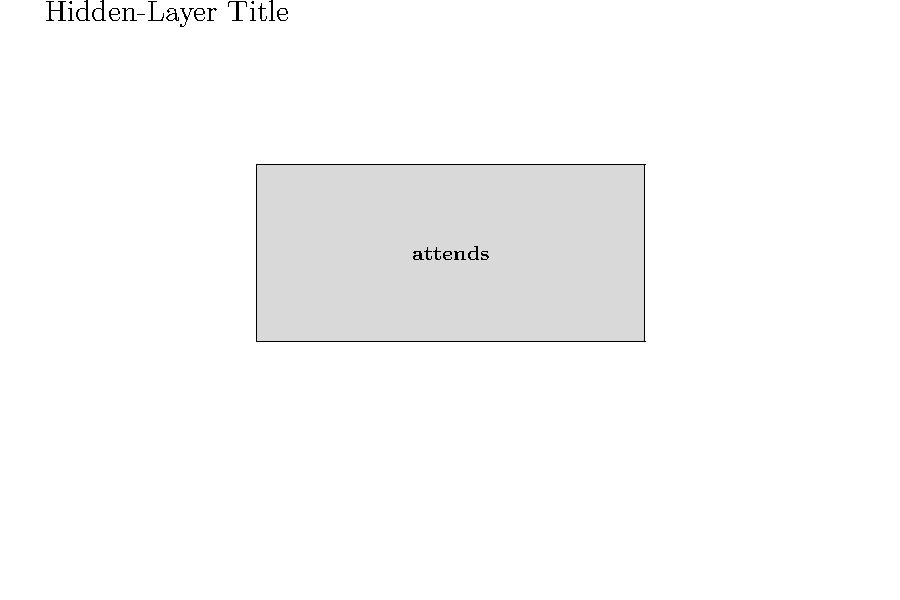
\includegraphics[viewport=90 40 330 200,clip,width=0.5\linewidth]{nips-grid-figure.pdf}
\caption{An example of the attention mechanism following long-distance dependencies.}
\end{figure}
\end{document}
